%+------------------------------------------------------------------------+
%| Diagram: Definition of Lie n-algebra of observables in a diagram
%| Author: Antonio miti
%+------------------------------------------------------------------------+


\documentclass[border=10pt, beamer]{standalone}

\usepackage{tikz}
\usetikzlibrary{arrows.meta, decorations.markings}
\usepackage{amssymb}

\begin{document}



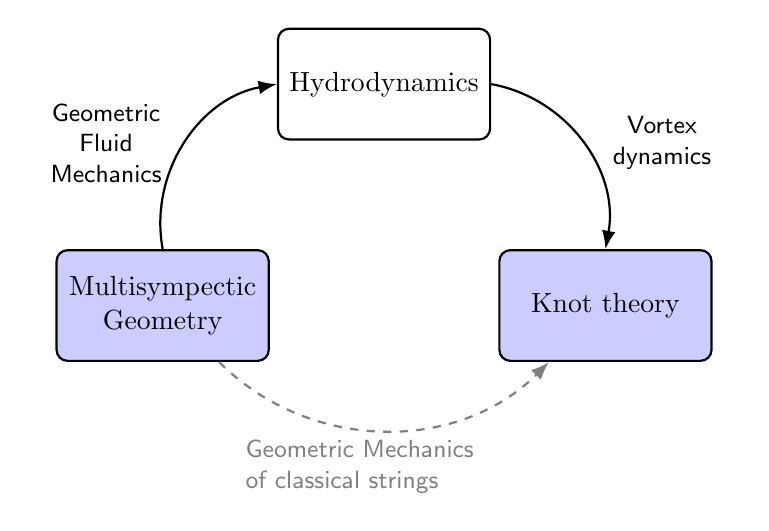
\begin{tikzpicture}[thick,node distance = 8em, auto]
    \node [->,rectangle, draw, fill=blue!20,
    text width=7em, text centered, rounded corners, minimum height=4em] (A)
    {Multisympectic Geometry};
    \node[inner sep=1em,minimum size=4em, text width=4em,right of=A] (k) {}; % invisible node
    \node [rectangle,above of=k, draw,
    text width=7em,text centered, rounded corners, minimum height=4em] (B)
    {Hydrodynamics};
    \node [rectangle,right of=k, draw, fill=blue!20, 
    text width=7em, text centered, rounded corners, minimum height=4em] (C)
    {Knot theory};
    
		\path[every node/.style={font=\sffamily\small}]
    	(A) edge[bend left=45,-Latex] node [left,text width=5em,align=center] {Geometric\\ Fluid\\ Mechanics} (B)
    	(B) edge[bend left=45,-Latex] node [right,text width=5em,align=center] {Vortex\\ dynamics} (C) ;
		\onslide<2->{\path[every node/.style={font=\sffamily\small}]
		    (A) edge[bend right=45,dashed,-Latex,gray] node [below,text width=10em] {Geometric Mechanics \\ of classical strings} (C);}
\end{tikzpicture}

\end{document}